\section{Results}
\label{sec:results}

% I write the description of the plots in their caption. In a succesive step of the work we can move the plot descriptions in the text. 

\begin{figure} [h!]
	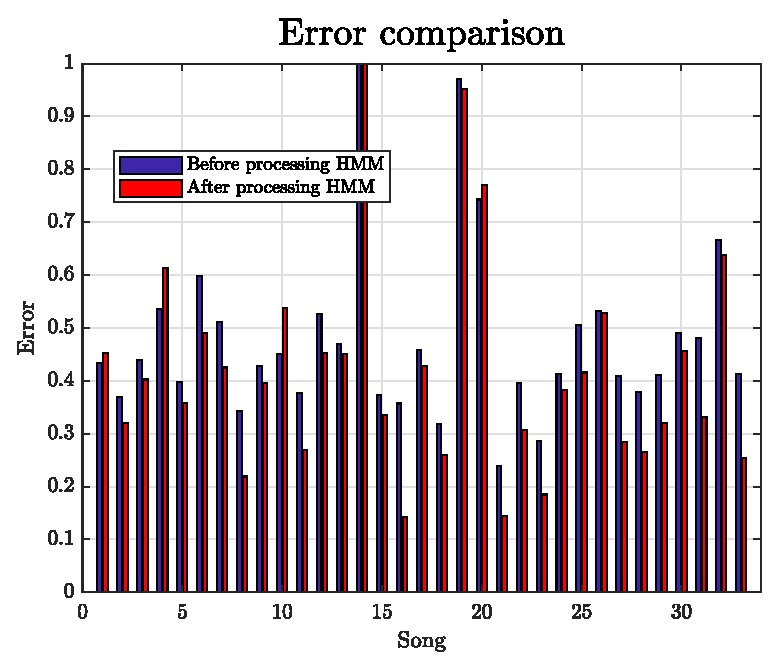
\includegraphics[width=0.5\textwidth]{img/Result_HMM/CENS/plot03071}
	\caption{Error comparison using CENS features (train = 0.7; test = 0.3). It is the one that has given the best results. We notice that a lot of songs have been discarded by Viterbi and therefore we have only 33 songs (not 150*0.3=45 as expected)}
\end{figure}

\begin{figure} [h!]
	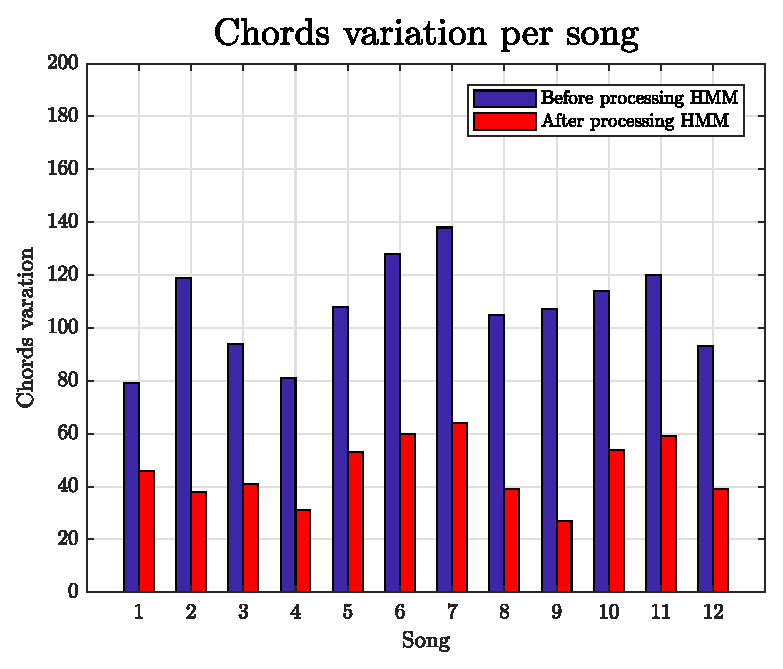
\includegraphics[width=0.5\textwidth]{img/Result_HMM/SMOOTHING/SmoothPerSongCENS0109}
	\caption{Chords variation per song using CENS features (train = 0.9; test = 0.1)}
\end{figure}

\begin{figure} [h!]
	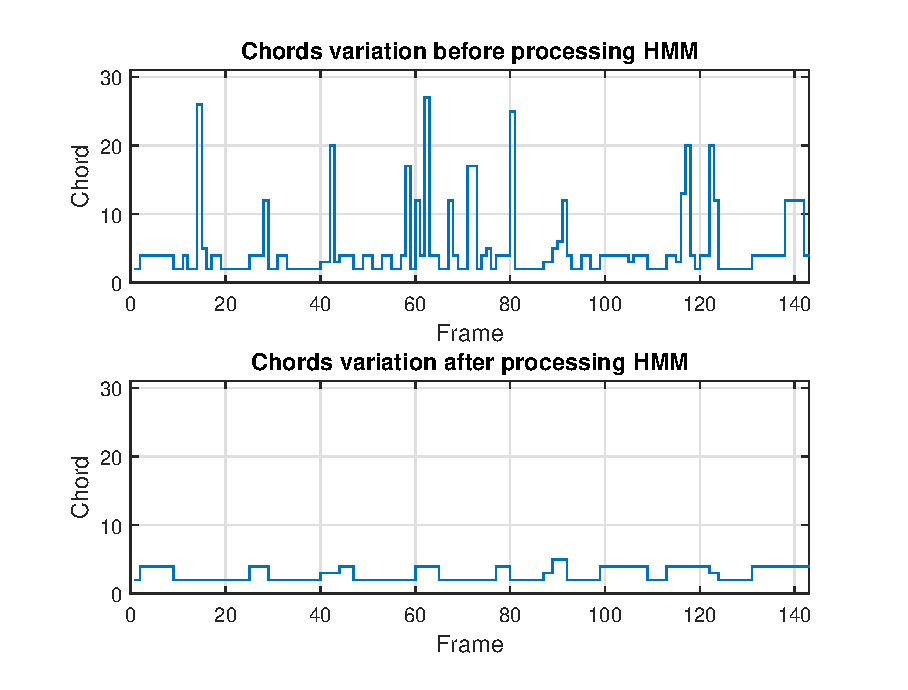
\includegraphics[width=0.5\textwidth]{img/Result_HMM/SMOOTHING/SmoothSingleSongCENS0109}
	\caption{Chord variation in a single song using CENS features (train = 0.9; test = 0.1); it represents the second song of the plot of the smoothing of all song}
\end{figure}
